  \section[Cloud]{Le Cloud : vue d'ensemble}

  \subsection[Cloud]{Le Cloud : les concepts}

  \begin{frame}
    \frametitle{Le cloud ? Vaste sujet !}
    \begin{itemize}
      \item Puissance de calcul, capacité de stockage et fonctionnalités réseau sous forme de services en-ligne\pause
      \item Flexibilité et élasticité des infrastructures\pause
      \item Libre-service, notion de catalogue\pause
      \item Accès en mode programmatique par des APIs, automatisation\pause
      \item Facturation à l'usage
    \end{itemize}
  \end{frame}

  \begin{frame}
    \frametitle{WaaS : Whatever as a Service}
    \begin{itemize}
      \item Principalement :
      \pause
      \begin{description}
        \item[IaaS] $\rightarrow$ \alert<5->{Infrastructure as a Service}\pause
        \item[PaaS] $\rightarrow$ Platform as a Service\pause
        \item[SaaS] $\rightarrow$ Software as a Service\pause
      \end{description}
      \pause
      \item Mais aussi :
      \pause
      \begin{itemize}
        \item Object Storage as a Service\pause
        \item Database as a Service\pause
        \item Load Balancing as a Service\pause
        \item DNS as a Service\pause
        \item \$Application as a Service
      \end{itemize}
    \end{itemize}
  \end{frame}

  \begin{frame}
    \frametitle{Cloud public, cloud privé, cloud hybride ?}
    \begin{description}
      \item[Public] $\rightarrow$ services cloud proposés par un fournisseur externe (AWS, Rackspace, OVS,...)\pause
      \item[Privé] $\rightarrow$ services cloud proposés par une entreprise/organisation à ses propres départements\pause 
      \item[Hybride] $\rightarrow$ utilisation des services d'un ou plusieurs clouds publics au sein d'un cloud privé
    \end{description}
  \end{frame}

  \begin{frame}
    \frametitle{Le cloud en un schéma}
    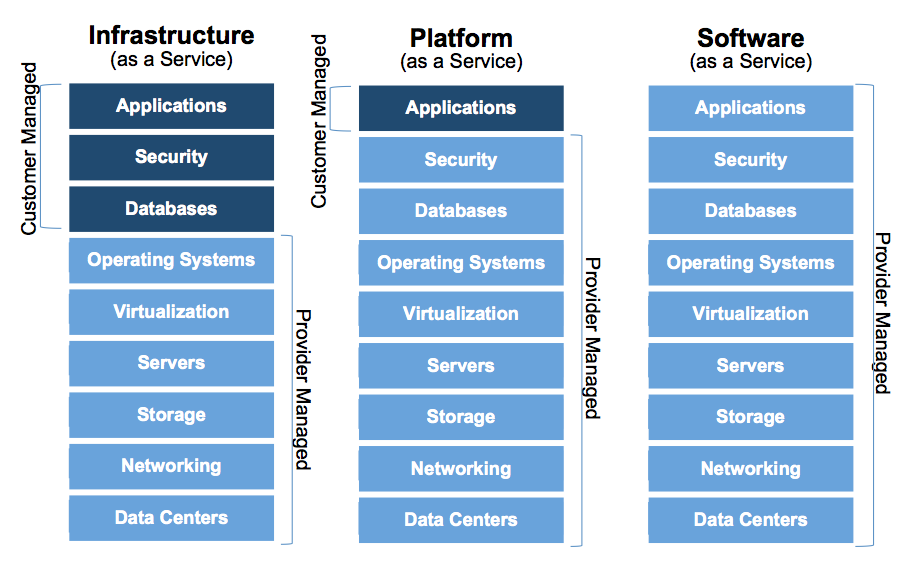
\includegraphics[width=\linewidth,height=\textheight]{images/cloud.png}
  \end{frame}

  \begin{frame}
    \frametitle{Pourquoi migrer vers le cloud ? Motivations d'ordre économique}
    \begin{itemize}
      \item appréhender les ressources IT comme des services "fournisseur"\pause
      \item réduire les coûts en mutualisant les ressources\pause
      \item réduire les délais d'approvisionnement de ressources\pause
      \item faire glisser le budget "investissement" (Capex) vers le budget "fonctionnement" (Opex)\pause
      \item aligner les coûts sur la consommation réelle des ressources\pause
      \item automatiser les opérations sur le SI et le rendre ainsi plus flexible
    \end{itemize}
  \end{frame}

  \begin{frame}
    \frametitle{Pourquoi migrer vers le cloud ? Motivations d'ordre technique}
    \begin{itemize}
      \item abstraire les couches basses (serveur, réseau, os, stockage)
      \pause
      \item s'affranchir de l'administration technique des ressources et services (BdD, pare-feux, load balancing,...)
      \pause
      \item concevoir des infrastructures scalables à la volée
      \pause
      \item agir sur les ressources via des lignes de code et gérer les infrastructures "comme du code".
    \end{itemize}
  \end{frame}

  \subsection[PaaS]{PaaS : Platform as a Service}

  \begin{frame}
    \frametitle{PaaS : concept d'application managée}
    \begin{itemize}
      \item Fourniture d'une plate-forme de "build, deploy and scale"
      \pause
      \item Pour un langage / un framework (python, java, php,...)
      \pause
      \item Principalement utilisé par des développeurs d'applications
    \end{itemize}
  \end{frame}

  \begin{frame}
    \frametitle{Exemples de PaaS public}
    \begin{itemize}
      \item Amazon Elastic Beanstalk (https://aws.amazon.com/fr/elasticbeanstalk)
      \pause
      \item Google App Engine (https://cloud.google.com/appengine)
      \pause
      \item Heroku (https://www.heroku.com)
    \end{itemize}
  \end{frame}

  \begin{frame}
    \frametitle{Solutions de PaaS privé}
    \begin{itemize}
      \item Cloud Foundry (https://www.cloudfoundry.org)
      \pause
      \item OpenShift (http://www.openshift.org)
      \pause
      \item \alert<5->{Solum} (https://wiki.openstack.org/wiki/Solum)
    \end{itemize}
  \end{frame}

  \subsection[IaaS]{IaaS : Infrastructure as a Service}

  \begin{frame}
    \frametitle{Le leader du IaaS public : Amazon Web Services (AWS)}
    \begin{itemize}
      \item Pionnier du marché (dès 2006)
      \pause
      \item Elastic Compute Cloud (\textcolor{blue}{EC2})\pause $\rightarrow$ puissance de calcul
      \pause
      \item Elastic Block Storage (\textcolor{blue}{EBS})\pause $\rightarrow$ stockage bloc
      \pause
      \item Simple Storage Service (\textcolor{blue}{S3})\pause $\rightarrow$ stockage objet
    \end{itemize}
  \end{frame}

  \begin{frame}
    \frametitle{Les clouds publics concurrents d'AWS}
    \begin{itemize}
      \item dans le monde :
      \begin{itemize}
        \item Google Compute Platform
        \item Microsoft Azure
        \item \textbf<3->{Rackspace}
      \end{itemize}
      \item en France :
      \begin{itemize}
        \item \textbf<3->{Cloudwatt} (Orange Business Services)
        \item \textbf<3->{Numergy} (SFR)
        \item Outscale
        \item \textbf<3->{OVH}
        \item Ikoula
        \item \textbf<3->{Scaleway (Iliad)}
      \end{itemize}
    \end{itemize}
  \end{frame}

  \begin{frame}
    \frametitle{Logiciels libres permettant le déploiement d'un cloud privé}
    \begin{itemize}
        \item Eucalyptus\pause
        \item CloudStack\pause
        \item OpenNebula\pause
        \item \textbf{OpenStack} (https://www.openstack.org)
    \end{itemize}
  \end{frame}

  \begin{frame}
    \frametitle{Correspondance OpenStack - AWS}
    \begin{table}[bt]
      \begin{tabular}{|l|c|c|} \hline
        \textbf{Service}      & \textbf{OpenStack}
                              & \textbf{AWS} \\ \hline
        \uncover<2->{compute} & \uncover<2->{Nova}
                              & \uncover<2->{EC2} \\
        \uncover<2->{block storage} & \uncover<2->{Cinder}
                              & \uncover<2->{EBS} \\
        \uncover<2->{object storage} & \uncover<2->{Swift}
                              & \uncover<2->{S3} \\ \hline
      \end{tabular}
    \end{table}
  \end{frame}

  \begin{frame}
    \frametitle{Virtualisation dans le cloud}
    \begin{itemize}
      \item Un cloud IaaS repose souvent sur la virtualisation
      \item Ressources "compute" $\leftarrow$ virtualisation
      \item Hyperviseurs : KVM, Xen (libvirt), ESX
      \item Conteneurs : OpenVZ, LXC, Docker, Kubernetes
    \end{itemize}
  \end{frame}

  \begin{frame}
    \frametitle{Notions et vocabulaire IaaS 1/4}
    \begin{itemize}
      \item Identité et accès
      \begin{itemize}
        \item Tenant/Projet (Project) : \pause locataire du cloud, propriétaire de ressources.
        \item Utilisateur (User) : \pause compte autorisé à utiliser les API OpenStack.
        \item Quota : \pause contrôle l'utilisation des ressources (vcpu, ram, fip, security groups,...) dans un tenant.
        \item Catalogue (de services) : \pause services disponibles et accessibles via les API.
        \item Endpoint : \pause URL permettant l'accès à une API. Un endpoint par service.
      \end{itemize}
    \end{itemize}
  \end{frame}

  \begin{frame}
    \frametitle{Notions et vocabulaire IaaS 2/4}
    \begin{itemize}
      \item Puissance de calcul, serveurs (Compute)
      \begin{itemize}
        \item Image : \pause
        \item Instance : \pause forme dynamique d'une image
        \item Type d'instance (flavor) : \pause définit les mensurations d'une instance (cpu, ram, capacité disque,...)
        \item Metadata et user data : \pause
        \item Cloud-init, cloud-config : \pause
      \end{itemize}
    \end{itemize}
  \end{frame}

  \begin{frame}
    \frametitle{Notions et vocabulaire IaaS 3/4}
    \begin{itemize}
      \item Stockage (Storage)
      \begin{itemize}
        \item Disque éphémère (Ephemeral disk) : \pause
        \item Volume : \pause disque virtuel en-ligne accessible par les instances
        \item Conteneur (Container) : \pause entités logiques pour le stockage de fichiers et accessibles via une URL
      \end{itemize}
      \item Réseau et sécurité (Network, Security)
      \begin{itemize}
        \item Groupe de sécurité (Security groups) : \pause ensemble de règles de filtrage de flux appliqué à l'entrée des instances.
        \item Paire de clés (Keypairs) : \pause
        \item IP flottantes (Floating IP) : \pause
      \end{itemize}
    \end{itemize}
  \end{frame}

  \begin{frame}
    \frametitle{Notions et vocabulaire IaaS 4/4}
    \begin{itemize}
      \item Orchestration
      \begin{itemize}
        \item Stack, template : \pause
      \end{itemize}
    \end{itemize}
  \end{frame}

  \begin{frame}
    \frametitle{OpenStack}
    \huge{Horizon, la console web d'OpenStack}
  \end{frame}

  \subsection[Orchestration]{Orchestrer les ressources de son IaaS}

  \begin{frame}
    \frametitle{Pourquoi orchestrer}
    \begin{itemize}
      \item Définir tout une infrastructure dans un seul fichier texte
      \item Être en capacité d'instancier une infrastructure entière en un appel API
      \item Autoscaling
      \begin{itemize}
        \item Adapter ses ressources en fonction de ses besoins en temps réel
        \item Fonctionnalité incluse dans le composant d'orchestration d'OpenStack
      \end{itemize}
    \end{itemize}
  \end{frame}

  \subsection[APIs]{APIs : quel rôle ?}

  \begin{frame}
    \frametitle{API ?}
    \begin{itemize}
      \item \textit{Application Programming Interface}
      \item Au sens logiciel : Interface permettant à un logiciel d'utiliser une bibliothèque
      \item Au sens cloud : Interface permettant à un logiciel d'utiliser un service (XaaS)
      \item Il s'agit le plus souvent d'API HTTP REST
    \end{itemize}
  \end{frame}

  \begin{frame}[containsverbatim]
    \frametitle{Exemple concret}
\begin{verbatim}
GET /v2.0/networks/<network_id>
{
   "network":{
      "status":"ACTIVE",
      "subnets":[
         "54d6f61d-db07-451c-9ab3-b9609b6b6f0b"
      ],
      "name":"private-network",
      "provider:physical_network":null,
      "admin_state_up":true,
      "tenant_id":"4fd44f30292945e481c7b8a0c8908869",
      "provider:network_type":"local",
      "router:external":true,
      "shared":true,
      "id":"d32019d3-bc6e-4319-9c1d-6722fc136a22",
      "provider:segmentation_id":null
   }
}
\end{verbatim}
  \end{frame}

